\documentclass[titlepage,a4paper,10pt]{article}
\usepackage{datetime,geometry,fancyhdr,lastpage,tabularx,color,paralist,makecell,tikz, listings, color, graphicx, float}
\usepackage[hidelinks]{hyperref}
\setcounter{tocdepth}{1}
% \usetikzlibrary{shapes.misc}
\usepackage[parfill]{parskip}
%\usepackage[nottoc,numbib]{tocbibind}
\usepackage[backend=biber,sorting=none]{biblatex}
% \addbibresource{/home/cfp/AUDrivesLocal/Admin/Templates/Latex/CFP/Bibliographies/cfp_bibliography.bib} %Put relevant bib resource here
%\settocbibname{References}
% \input{cfp_latex_settings.tex}
%\usepackage{fullpage, comment, bookman}
\pagestyle{fancy} \fancyhf{} \renewcommand{\headrulewidth}{0pt} \cfoot{\thepage\ of \pageref{LastPage}}

\setlength\parindent{0pt}

\newcommand{\red}[1]{\textcolor{red}{#1}}
\newcommand{\green}[1]{\textcolor{green}{#1}}

\tikzset{blue node/.style={circle,fill=blue!20,draw,minimum size=1cm,inner sep=4pt},}
\tikzset{white node/.style={circle,fill=white,draw,minimum size=1cm,inner sep=4pt},}
\tikzset{blue node double/.style={circle,fill=blue!20,draw,double, double distance=1mm, minimum size=1cm,inner sep=4pt},}
\tikzset{white node double/.style={circle,fill=white,draw,double, double distance=1mm, minimum size=1cm,inner sep=4pt},}

%\specialcomment{answer}{\begingroup \color{blue}}{\endgroup}
%\newcommand{\mystar}{\hspace{-2em}{$\star$}\hspace{1.5em}}
%\%includecomment{comment}

\begin{document}

\title{Distributed Systems \\3rd Semester, BSc, Computer Engineering, AU\\~\\Project Description: \\Chinese Fortune Cookies}
\author{Christian Marius Lillelund, cl@eng.au.dk}
\date{\today, \currenttime\\
  \vfill
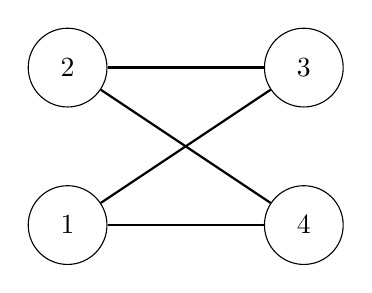
\begin{tikzpicture}
 %% Nodes
  \node[white node] (1) at (0,0) {1};
  \node[white node] (2) at (0,2) {2};
  \node[white node] (3) at (3,2) {3};
  \node[white node] (4) at (3,0) {4};
  %% Paths
  \path[draw,thick]
    (1) edge node {} (4)
    (1) edge node {} (3)
    (4) edge node {} (2)
    (2) edge node {} (3);
\end{tikzpicture}
}
\maketitle

%\tableofcontents

%\newpage
\section{Background}

Much to people's surprise, the fortune cookie is not a Chinese invention, but an American fancy originating in California. It is often served as a dessert in Chinese restaurants in the United States and other Western countries.

\section{Problem formulation}

In this exercise you'll get a chance to offer people an infinite amount of fortune cookies by just clicking a button. You'll use Kubernetes to create a backend service that'll return a fortune cookie upon request. You can store these cookies in memory, in a file you include in your Dockerfile or on the Internet. If you need some cookies, look in Appendix A. The website can be a simple HTML page, some CSS styling and a bit of JavaScript that fetches a cookie from your API whenever the user presses a button.

Formally, your solution should contain at least:

\begin{itemize}
	\item A deployment specification that supports multiple pods and has resources enabled.
	\item A service that can forward HTTP calls to your pods. 
	\item A website with some visualization of the cookie text and a way to get more (see figure \ref{fig:fortunecookie}).
\end{itemize}

Also, you must conduct the following experiments and support your findings with measurements and your own arguments:

\begin{itemize}
	\item Run a load test towards your Kubernetes service with a different number of active replica pods, for example 2, 5, and 10, and write down your results. You can use PowerShell or NodeJS to make a simple loop that sends a lot of HTTP requests rapidly to your endpoint. Do you notice any lag? Does response times improve when you add more pods? Why or why not?
	\item With memory and CPU resources enabled for pods, experiment with various settings. What happens if you set the CPU resources very low? What happens if a container exceeds its memory limit? Document your findings.
\end{itemize}

For help with resources, see: \\ \url{https://kubernetes.io/docs/concepts/configuration/manage-resources-containers/}

\begin{figure}[H]
	\centering
	\fbox{\includegraphics[width=0.7\linewidth]{fortune_cookie}}
	\caption{How your fortune cookie website could look.}
	\label{fig:fortunecookie}
\end{figure}

\pagebreak

\appendix
\section{Cookies}

"Today it's up to you to create the peacefulness you long for.", \\
"A friend asks only for your time not your money.", \\
"If you refuse to accept anything but the best, you very often get it.",\\
"A smile is your passport into the hearts of others.",\\
"A good way to keep healthy is to eat more Chinese food.",\\
"Your high-minded principles spell success.",\\
"Hard work pays off in the future, laziness pays off now.",\\
"Change can hurt, but it leads a path to something better.",\\
"Enjoy the good luck a companion brings you.",\\
"People are naturally attracted to you.",\\
"Hidden in a valley beside an open stream- This will be the type of place where you will find your dream.",\\
"A chance meeting opens new doors to success and friendship.",\\
"You learn from your mistakes... You will learn a lot today.",\\
"If you have something good in your life, don't let it go!",\\
"What ever you're goal is in life, embrace it visualize it, and for it will be yours.",\\
"Your shoes will make you happy today.",\\
"You cannot love life until you live the life you love.",\\
"Be on the lookout for coming events; They cast their shadows beforehand.",\\
"Land is always on the mind of a flying bird.",\\
"The man or woman you desire feels the same about you.",\\
"Meeting adversity well is the source of your strength.",\\
"A dream you have will come true.",\\
"Our deeds determine us, as much as we determine our deeds.",\\
"Never give up. You're not a failure if you don't give up.",\\
"You will become great if you believe in yourself.",\\
"There is no greater pleasure than seeing your loved ones prosper.",\\
"You will marry your lover.",\\
"A very attractive person has a message for you.",\\
"You already know the answer to the questions lingering inside your head.",\\
"It is now, and in this world, that we must live.",\\
"You must try, or hate yourself for not trying.",\\
"You can make your own happiness."

\newpage
\printbibliography[heading=bibintoc, resetnumbers=true]

\end{document}


